\label{chapter:experiments}
\chapter{Benchmarking and Performance Regression}

By quantifying user experience, we can try to understand it better and improve it. This chapter will focus on experiments that are measuring the performance of the Tribler core, with a particular focus on user experience. Various common operations executed by users in Tribler are identified, discussed and measured.

\section{Experiments environment}
The experiments with the Tribler core are performed on a virtual private server. We tried to keep close to the specifications of a machine that an actual user could be using. The virtual server has 8GB of memory and 1 processor with 4 cores (with a clock speed of 2,5GHz). The used operation system is Ubuntu 15.10.\\\\
If not stated otherwise, the default values of the Tribler configuration file are used. These default values can be found in the `defaults.py` file in the source code directory of Tribler\footnote{https://github.com/Tribler/tribler/blob/devel/Tribler/Core/defaults.py}. All communities, except for \emph{Multichain} and \emph{BarterCast}, are loaded.

\section{Start-up experience}
The very first interaction that users have with Tribler, is the process of starting. During the boot process, various operations are performed:
\begin{itemize}
	\item The connection to the sqlite database is opened and initialized. If this database does not exist, it will be created.
	\item Dispersy is started and the enabled communities are loaded.
	\item Various Tribler components are created, including the video streaming server, the REST API, the remote torrent handler and the \emph{leveldb} store.
\end{itemize}
The start-up process of the Tribler core happens sequentially and no parallel operations are in place to speed up the process. Depending on the number of enabled components, the start-up time might vary.\\\\
To analyse the start-up time, Tribler is started 30 times. In half of the runs, the software is started for the first time, with no prior existing state directory. In these runs, a state directory is created and the required files are initialized. In the other half of the runs, a database with a little over 100.000 torrents is used. This database is the result of running Tribler idle for several hours, after subscribing to some popular channels. Moreover, a filled Dispersy database is used for the second half of the runs. In both scenarios, there are no downloads running. The experiment starts when the \emph{start} method of the \emph{Session} object is called and ends when the notification that Tribler has started, is observed. The results are displayed in Figure \ref{fig:startup_experiment}.\\\\
It is clear that magnitudes of the Tribler and Dispersy databases have impact on the time for Tribler to completely start. However, this impact is relatively minor since Tribler still starts within a second. We think that this statistic justifies removal of the splash screen that is shown in the old user interface. The relatively short time the splash screen would be visible in the new interface is so short that users would not even be able to read and interpret the content of the splash screen.\\\\
In both plots, some outliers are present. Further analysis learns us that these variations are caused by the loading process of the Dispersy communities, however, further investigation of the initialization part of Dispersy is considered future work.

\begin{figure}[!h]
	\centering
	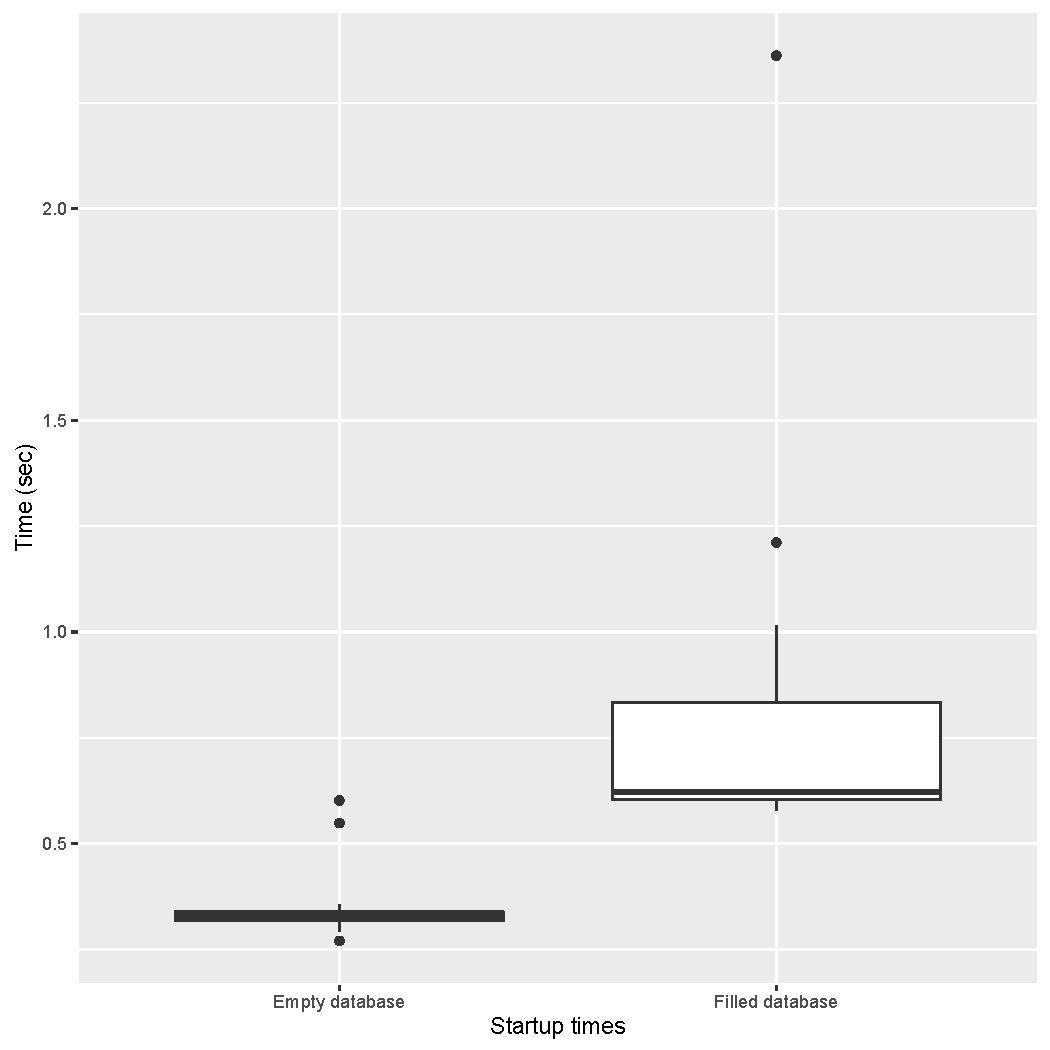
\includegraphics[width=0.6\columnwidth]{images/experiments/startup}
	\caption{Test.}
	\label{fig:startup_experiment}
\end{figure}

\section{Content Search}
We wish to serve relevant information to users as fast as possible. To help users search for relevant content, a remote keyword search has been implemented. Matching search results can either be torrents or channels. Channel results are fetched by a query in the \emph{AllChannel} community whereas torrent results are retrieved by a query in the \emph{search} community.\\\\
To verify the speed of the remote torrent search, various experiments are conducted. We are using a list of 100 terms that users might be searching for. This list of search terms can be found in Appendix x\todo{Add this}. Each query is executed when there are at least 20 connected peers in the \emph{SearchCommunity}. The timeout period of the remote search is 60 seconds. This experiment has a particular focus on two statistics: the time until the first remote torrent search results comes in and the turnaround time of the search request. We should note that users performing a remote search might see results earlier since in parallel, a  search query in the local database is performed. The results are visible in Figure \ref{fig:remote_search_first_result} and \ref{fig:remote_search_all_result}.\todo{nitin graph}\\\\
Overall, the remote torrent search as implemented in Tribler is very fast and performs well. On average, 61 search results are returned for each query and the first incoming torrent result takes 0.26 seconds to arrive. As we see in Figure \ref{fig:remote_search_first_result}, over 90\% of the first remote search results are available to the user within a second. During our experiment, we always have the first incoming torrent result within 3.5 seconds.\\\\
The other graphs shows the turnaround time of the request. On average, it takes 2.1 seconds for all torrent search results to arrive. From Figure \ref{fig:remote_search_all_result}, we see that in over 90\% of the search queries, we have all results within 10 seconds.

\begin{figure}[!h]
	\centering
	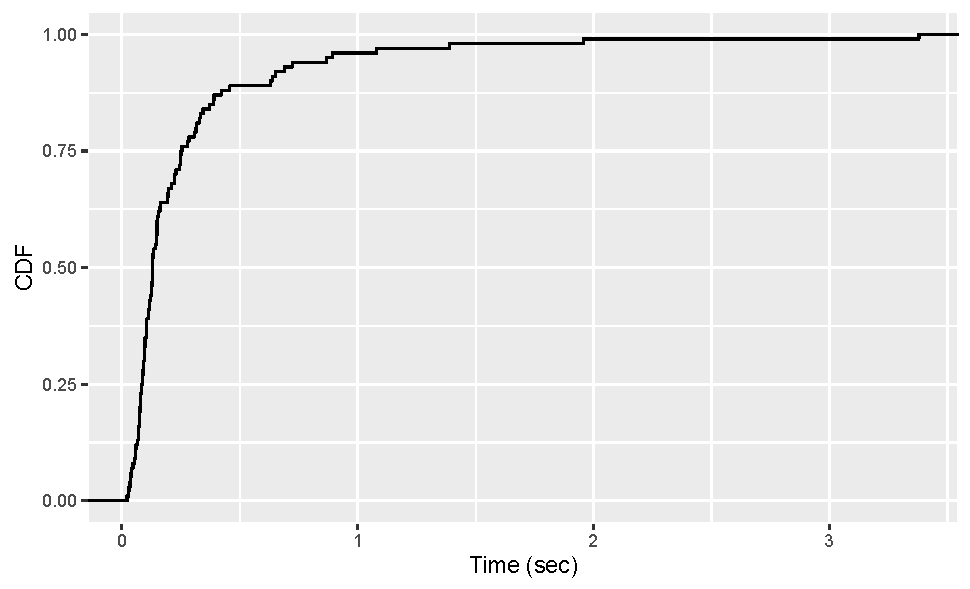
\includegraphics[width=0.6\columnwidth]{images/experiments/cdf_remote_search_first_results}
	\caption{Test.}
	\label{fig:remote_search_first_result}
\end{figure}

\begin{figure}[!h]
	\centering
	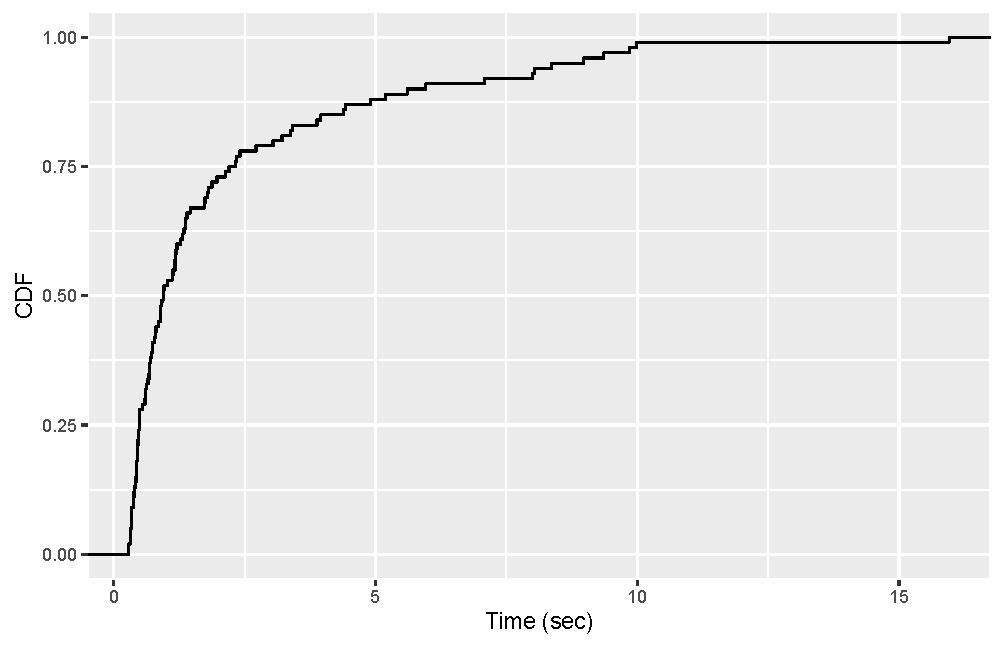
\includegraphics[width=0.6\columnwidth]{images/experiments/cdf_remote_search_all_results}
	\caption{Test.}
	\label{fig:remote_search_all_result}
\end{figure}

\section{Local keyword search}
...

\section{Video streaming}
...

\section{Content discovery}
...

\section{Channel subscription}
...

\section{Fetching metainfo of torrents}
...

\section{Profiling Tribler on low-end devices}
The addition of a REST API allows developers to have flexibility to run Tribler remotely, for instance, on embedded devices such as a Raspberry Pi. The running Tribler instance can be controlled from external devices by performing HTTP requests. Android is another example of a device that can run Tribler. During the last years, various research have been conducted to execute Tribler on Android devices\todo{cites}. Running Tribler on a low-end device, can yield much information about bottlenecks that might not be directly visible when running Tribler on a desktop or supercomputer.\\\\
The experiments described in this Section are executed on a Raspberry Pi, third generation with 1GB LPDDR2 ram, 4× ARM Cortex-A53, 1.2GHz CPU and 16GB storage on a microSD card. The used operating system is raspbian, the official system specifically designed for the Raspberry Pi, based on Debian.\\\\
Regular usage of Tribler on the Raspberry Pi using the REST API have us suspected that the Raspberry Pi is under heavy load. Monitoring the process for a while, reveals that the CPU usage is often around 100\%, completely filling up one CPU core. To get a detailed breakdown of execution time per method in the code base, the Yappi profiler has been used to analyse the performance of the Tribler session. This profiler has been integrated in the \emph{twistd} Tribler plugin and can be started together with Tribler by passing a flag when starting the plugin. The output of the profiler is a \emph{callgrind} file that can be loaded and analysed by third party software. The breakdown of a 20-minute run is visible in Figure x\todo{figure}.

\begin{figure}[!h]
	\centering
	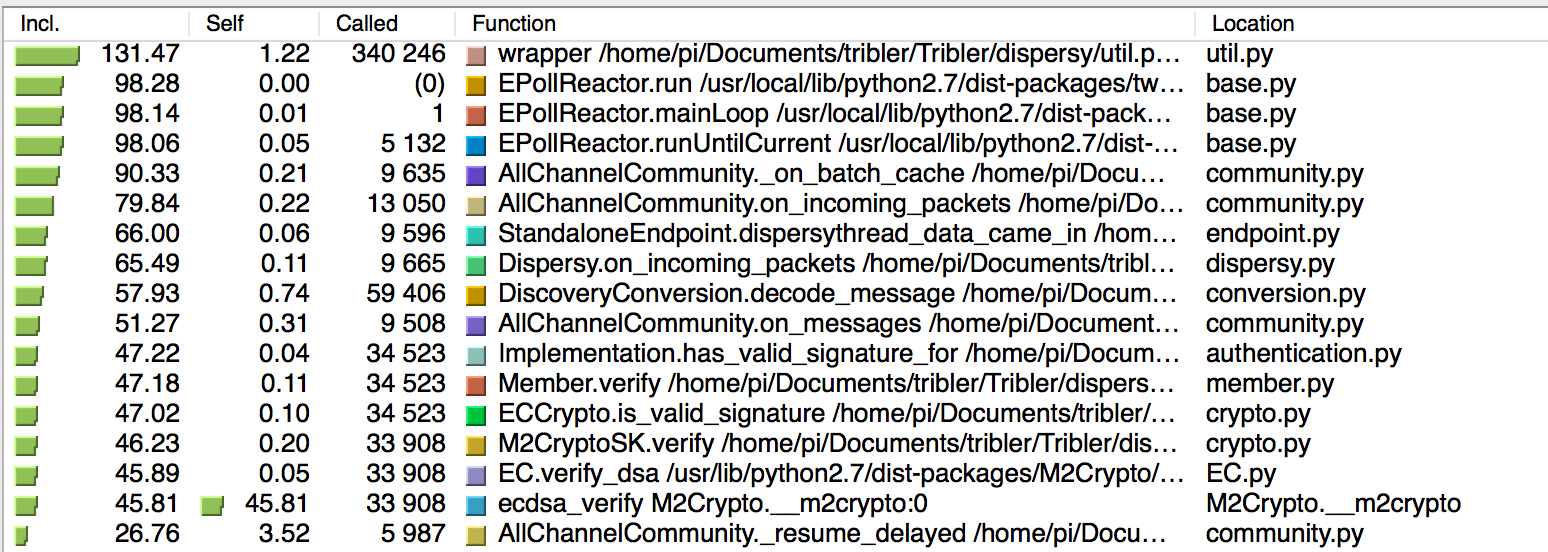
\includegraphics[width=0.9\columnwidth]{images/experiments/yappi_breakdown}
	\caption{Test.}
	\label{fig:yappi_breakdown}
\end{figure}

The file created by Yappi gives a detailed overview of the execution time of methods and can be used as a tool to detect performance bottlenecks in the system. The column \emph{Incl.} gives the inclusive cost of the function, this means the execution time of function itself and all it's including functions. The column \emph{self} gives only the execution time of the function, without considering callees. The other columns are self-explanatory and can be used to track the respective function in the source code.\\\\
From the breakdown, it is clear that Dispersy has a big impact on the performance of Tribler when running on the Raspberry Pi. The \emph{ecdsa\_verify} method is dominating the runtime of Tribler: the method is responsible for 45.81\% of the runtime. This specific method verifies the sign of an incoming Dispersy message and is invoked every time a signed message comes in. Disabling cryptographic verification of incoming messages should improve the situation, however, this is a trade-off between security and performance. By not verifying incoming messages, fake messages by an adversary can be forged and are accepted in such as system. To verify whether the responsiveness of the system improves, we measure the CPU usage of two runs. Both runs start with a non-existing Tribler state directory and have a duration of five minutes. In the first run, we are using the default configuration of Tribler, like in most of the other experiments in this Chapter. In the second run, we disable verification of incoming messages to see how things improve. The two runs are displayed in Figure \ref{fig:raspi_cpu_usage}.\\\\

\begin{figure}[!h]
	\centering
	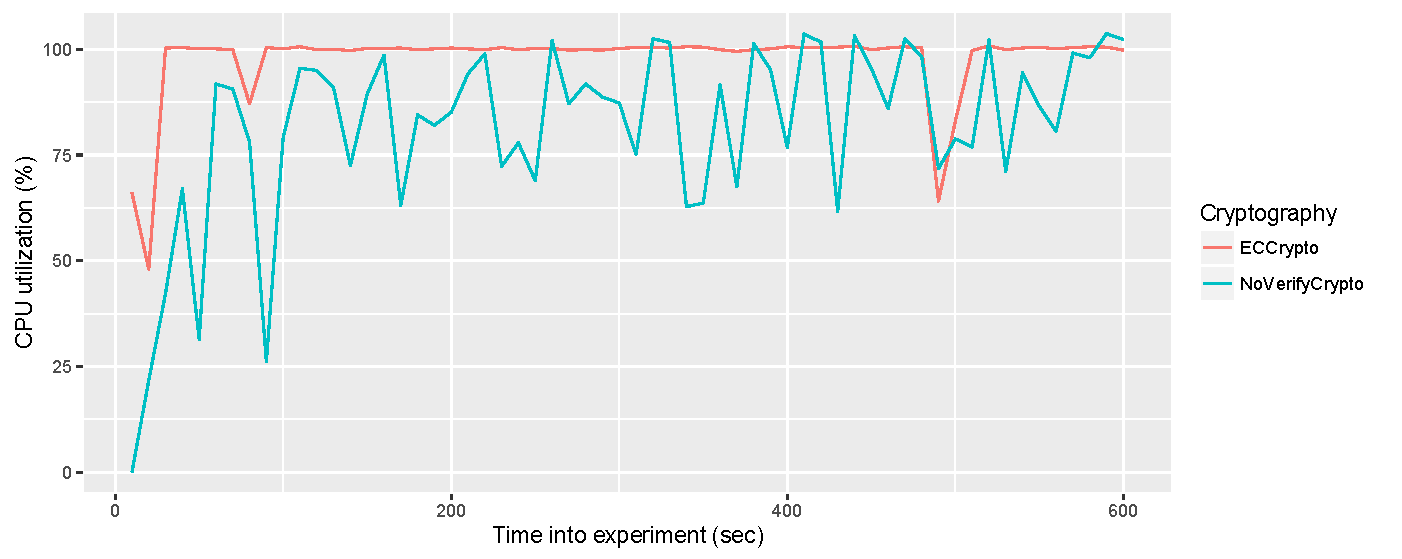
\includegraphics[width=1.0\columnwidth]{images/experiments/raspi_cpu_usage}
	\caption{Test.}
	\label{fig:raspi_cpu_usage}
\end{figure}

In the Figure, some occurrences are visible where the CPU usage appears to be over 100\%. This is explained by the fact that some of the underlying code is designed to run on multiple processors. While the threading model of Tribler is limited to a single core, the runtime and interpreter might execute code on additional cores. In the run where we enable all components of the system, the CPU usage is often 100\%. When verification of Dispersy messages is disabled, we see somewhat more drops in CPU usage but the utilization jumps back immediately to higher amounts. Disabling message verification is clearly not enough to guarantee a usable and responsive system.\\\\
To detect other performance bottlenecks, we sort the Yappi report on the \emph{Self} column to get insight in methods that are taking a long time to complete. This is visible in Figure \ref{fig:yappi_breakdown_self}. An interesting observation here is that the Python built-in \emph{all} method takes up a significant amount of time (6.13\% of the runtime). The \emph{all} method takes an iterable object and returns true if all objects of this collections are true. Both the \emph{all} method and \emph{zip} method (also visible in Figure \ref{fig:yappi_breakdown_self}) is used in the \emph{\_resume\_delayed} method. Optimization of this method is considered future work and described in GitHub issue 505\footnote{https://github.com/Tribler/dispersy/issues/505}.\\\\

\begin{figure}[!h]
	\centering
	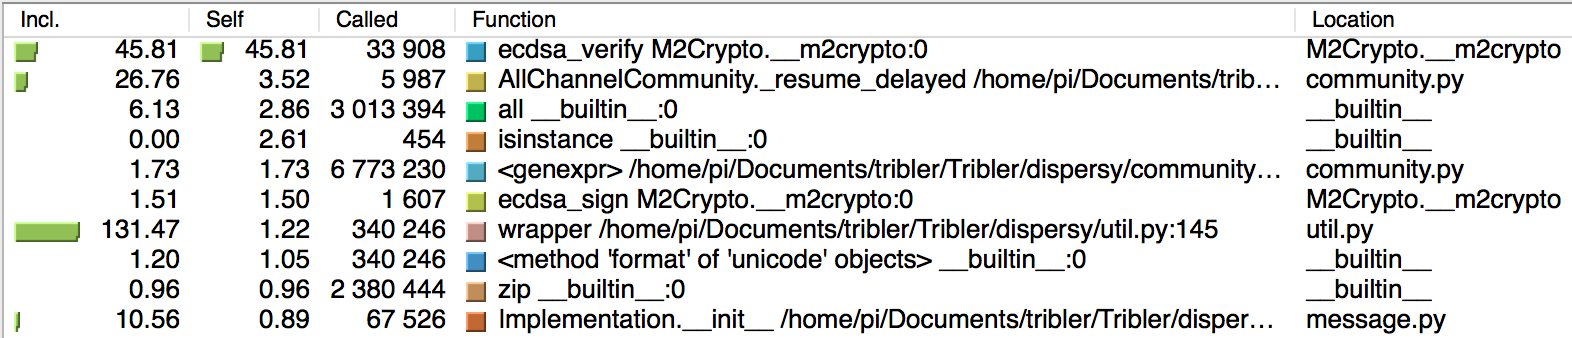
\includegraphics[width=0.9\columnwidth]{images/experiments/yappi_breakdown_self}
	\caption{Test.}
	\label{fig:yappi_breakdown_self}
\end{figure}

This shows that the Yappi profiler can be a very convenient tool to detect and track performance bottlenecks. The integration in the twistd plugin makes it easy for developers to run and analyse Tribler sessions under different circumstances.